%% --------------------------------------------------------------
% This is all preamble stuff that you don't have to worry about.
% Head down to where it says "Start here"
% --------------------------------------------------------------
 
\documentclass[12pt]{article} 
\usepackage[margin=1in]{geometry} 
\usepackage{bm} % bold in mathmode \bm
\usepackage{amsmath,amsthm,amssymb,mathtools}
\usepackage{dsfont} % for indicator function \mathds 1
\usepackage{tikz,pgf,pgfplots}
\usepackage{enumerate} 
\usepackage[multiple]{footmisc} % for an adjascent footnote
\usepackage{graphicx,float} % figures
\usepackage{framed} % surround a text with a box 
\usepackage{csvsimple,longtable,booktabs} % load csv as a table
\usepackage{listings,color} % for code snippets

\newtheorem{definition}{Definition}
\let\olddefinition\definition
\renewcommand{\definition}{\olddefinition\normalfont}
\newtheorem{lemma}{Lemma}
\let\oldlemma\lemma
\renewcommand{\lemma}{\oldlemma\normalfont}
\newtheorem{proposition}{Proposition}
\let\oldproposition\proposition
\renewcommand{\proposition}{\oldproposition\normalfont}
\newtheorem{corollary}{Corollary}
\let\oldcorollary\corollary
\renewcommand{\corollary}{\oldcorollary\normalfont}
\newtheorem{theorem}{Theorem}
\let\oldtheorem\theorem
\renewcommand{\theorem}{\oldtheorem\normalfont}

%%% PLOTTING PARAMETERS
\tikzstyle{bag} = [text width=7em, text centered] %binomial tree node width
\tikzstyle{end} = []
%%%

%% set noindent by default and define indent to be the standard indent length
\newlength\tindent
\setlength{\tindent}{\parindent}
\setlength{\parindent}{0pt}
\renewcommand{\indent}{\hspace*{\tindent}}

\newcommand*{\vv}[1]{\vec{\mkern0mu#1}} % \vec command

%% DAVIDS MACRO KIT %%
\newcommand{\R}{\mathbb R}
\newcommand{\N}{\mathbb N}
\newcommand{\Z}{\mathbb Z}
\renewcommand{\P}{\mathbb P}
\newcommand{\Q}{\mathbb Q}
\newcommand{\E}{\mathbb E}
\newcommand{\var}{\mathrm{Var}}
\newcommand{\Var}{\mathrm{Var}}
\newcommand{\cov}{\mathrm{Cov}}
\newcommand{\Cov}{\mathrm{Cov}}
\newcommand{\indist}{\,{\buildrel \mathcal D \over \sim}\,}

\newcommand{\bigtau}{\text{{\large $\bm \tau$}}}



 
%%======%%
% All this is to force LaTeX to prefix "Appendix" before a new appendix section letter
\makeatletter
% The "\@seccntformat" command is an auxiliary command
% (see pp. 26f. of 'The LaTeX Companion,' 2nd. ed.)
\def\@seccntformat#1{\@ifundefined{#1@cntformat}%
   {\csname the#1\endcsname\quad}  % default
   {\csname #1@cntformat\endcsname}% enable individual control
}
\let\oldappendix\appendix %% save current definition of \appendix
\renewcommand\appendix{%
    \oldappendix
    \newcommand{\section@cntformat}{\appendixname~\thesection\quad}
}
\makeatother
%%======%%

%%======%%
% Define for code section
\definecolor{dkgreen}{rgb}{0,0.6,0}
\definecolor{gray}{rgb}{0.5,0.5,0.5}
\definecolor{mauve}{rgb}{0.58,0,0.82}

\lstset{frame=tb,
  language=C++,
  aboveskip=3mm,
  belowskip=3mm,
  showstringspaces=false,
  columns=flexible,
  basicstyle={\footnotesize\ttfamily},
  numbers=none,
  numberstyle=\tiny\color{gray},
  keywordstyle=\color{blue},
  commentstyle=\color{dkgreen},
  stringstyle=\color{mauve},
  breaklines=true,
  breakatwhitespace=true,
  tabsize=3
}
%%======%%


\begin{document}
 
% --------------------------------------------------------------
%                         Start here
% --------------------------------------------------------------
 
\newpage
{\bf Part II.} \\

{\bf Question 1.} \\

\indent Presented in the figures below include the implied volatility plots for the given options written on Google stock. We note a decided `smile' in shape of the implied volatilities as a function of strike price. That is, contrary to the modelling assumption of constant volatilities, we find variable values for the volatilities as computed by the binomial model.

\begin{figure}[H]
	\centering
 	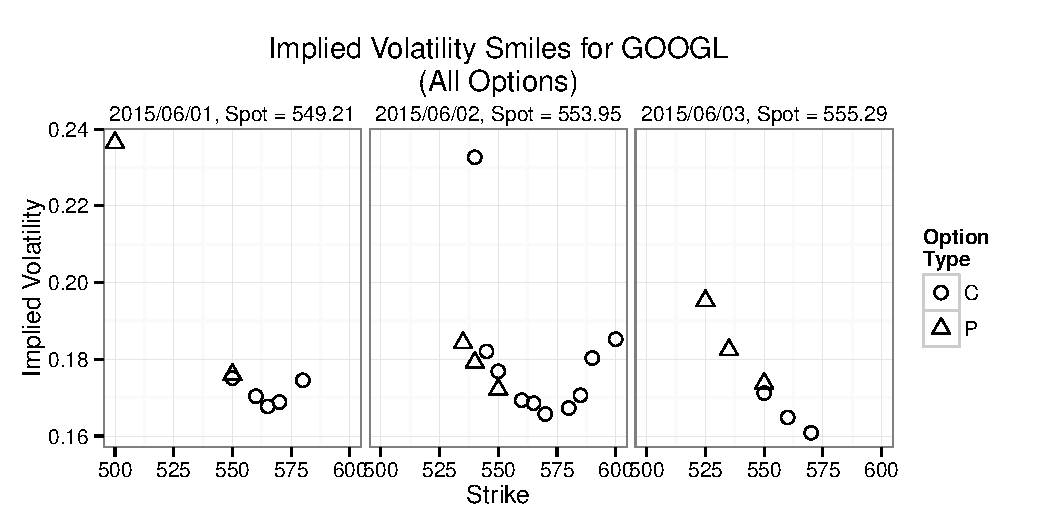
\includegraphics[scale=0.85]{../plots/smile_all.pdf}
\caption{\footnotesize Volatility smile(s) for all options written on GOOGL.}
\end{figure}

\begin{figure}[H]
	\centering
 	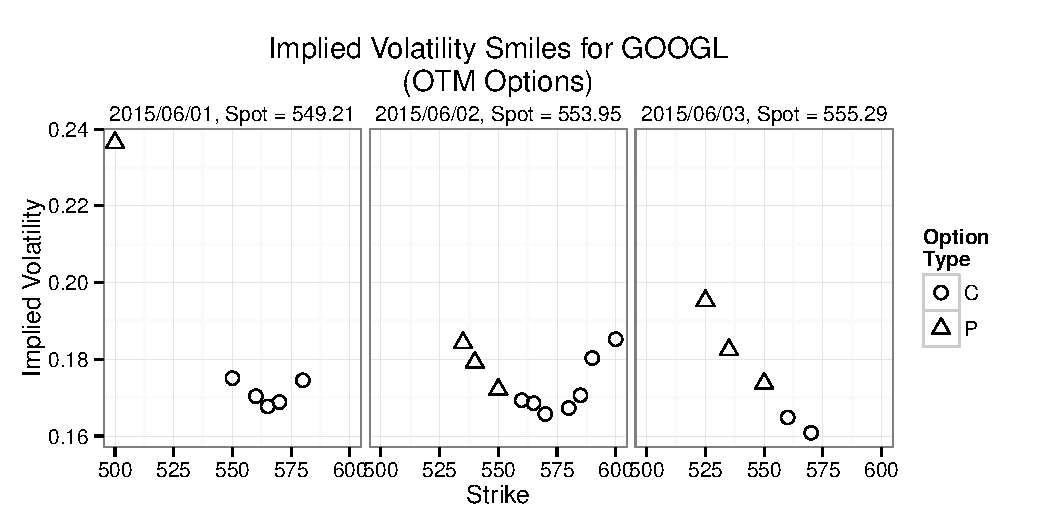
\includegraphics[scale=0.85]{../plots/smile_OTM.pdf}
\caption{\footnotesize Volatility smile(s) for OTM options written on GOOGL.}
\end{figure}


\indent If we were so daring as to examine the convergence of the binomial model we do indeed find a trend towards convergence relatively quickly. As illustrated by the figures below, given a four sampled options from the set of 26, by $N = 10^3$ we see little appreciable gain in volatility estimates. 

\begin{figure}[H]
	\centering
 	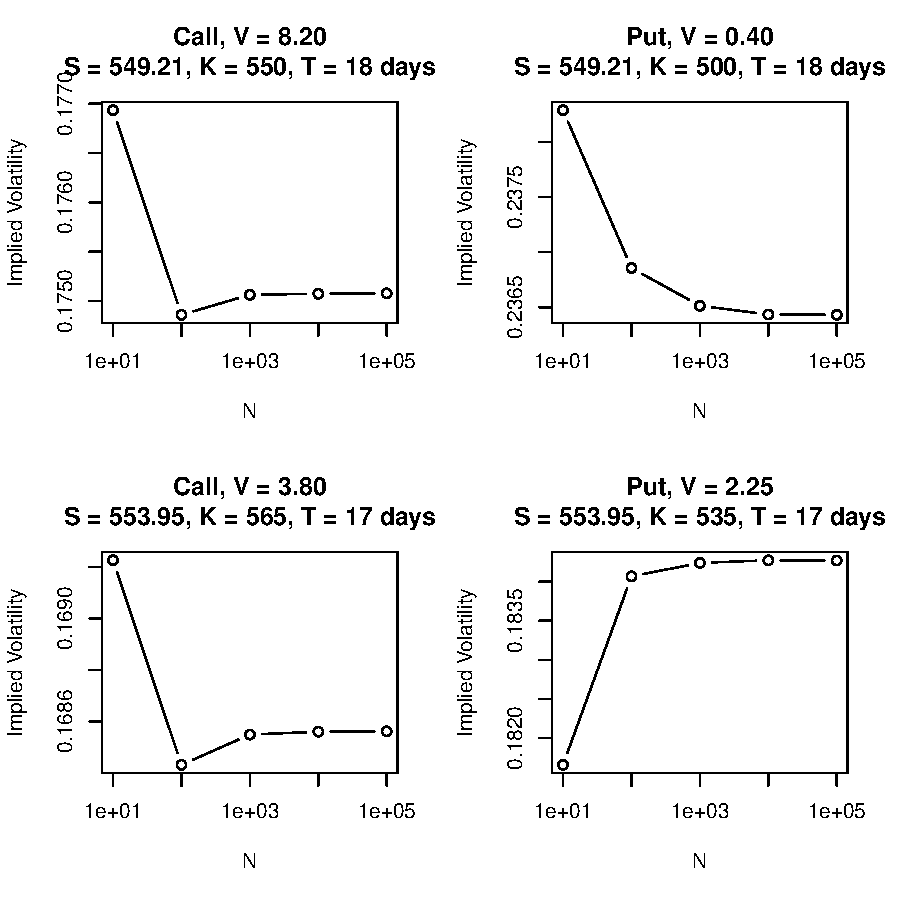
\includegraphics[scale=0.75]{../plots/imp_vol_conv_N.pdf}
\caption{\footnotesize Implied volatility estimates given call option strike prices as a function of the $N$-steps of the binomial model. Qualitatively, convergence appears to occur relatively rapidly: By $N = 10^3$ little gains to volatility precision occurs. }
\end{figure}

\indent However, examining the volatilities in question at such large intervals obfuscates some interesting behaviour of the binomial model. If we consider the model output while increasing the number of steps one at a time we find periodicity in our volatility estimates. For example, consider the figures below illustrating the first option in our list: A European call option with ask 8.20, spot price 549.21, strike price 550, with 18 days to expiry.

\begin{figure}[H]
	\centering
 	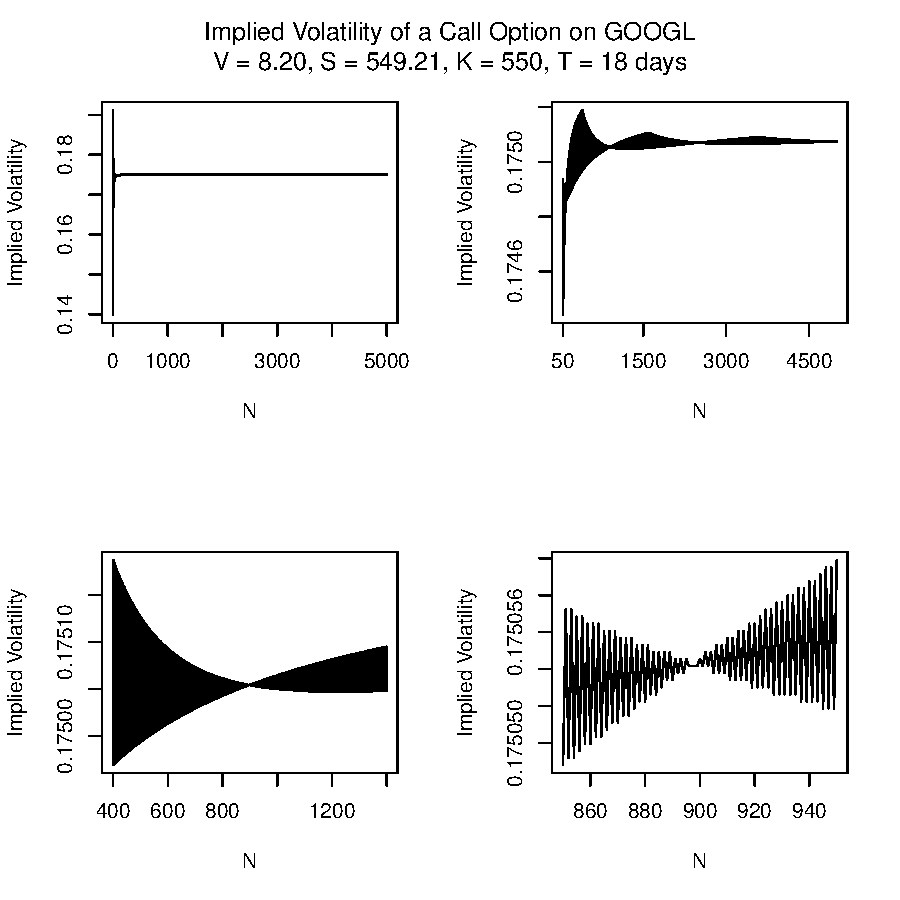
\includegraphics[scale=0.75]{../plots/imp_vol_conv.pdf}
\caption{\footnotesize Periodic behaviour seen in the values of the implied volatility as computed for the first option in our data set by the bisection algorithm.}
\end{figure}

\begin{figure}[H]
	\centering
 	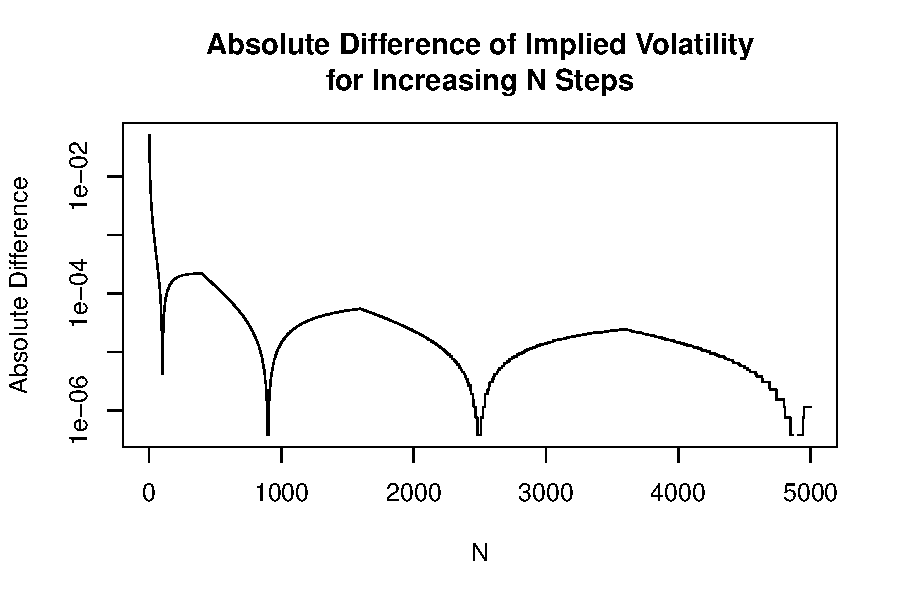
\includegraphics[scale=0.52]{../plots/imp_vol_conv_diff.pdf}
\caption{\footnotesize Increasing the value of $N$ leads to periodic behaviour in the additional precision for estimates of implied volatility, with a decreasing trend. Stepwise behaviour for large $N$ can be attributed to the cut-off of $|V_{obs} - V_{imp}| < 10^{-5}$ in the bisection and not the underlying model.}
\end{figure}

\indent To be sure that such periodicity is not attributable to the bisection algorithm, or some source other than the binomial model, we should also examine the output of the pricing algorithm a single step at a time. As an example, we consider the first option in our list: The same European call option with ask 8.20, spot price 549.21, strike price 550, with 18 days to expiry. To price an option we require a value for $\sigma$ and so for the sake of illustration we also assume a ``true'' value for the volatility parameter $\sigma$ to be 0.17507.


\begin{figure}[H]
	\centering
 	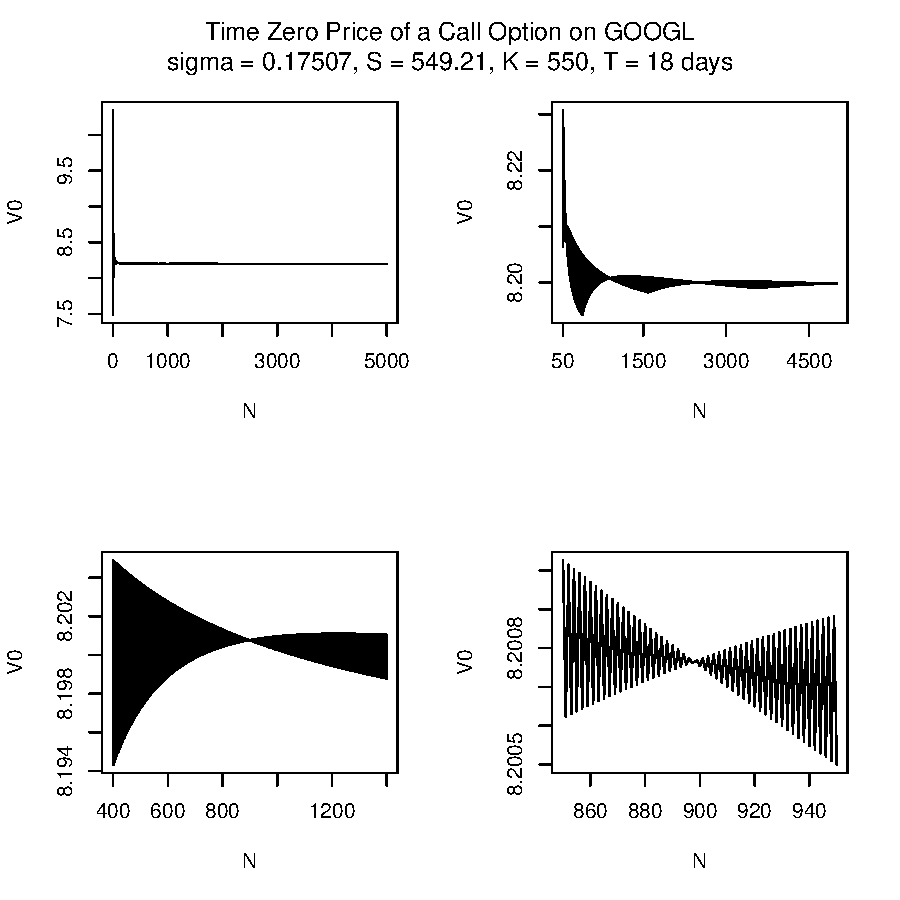
\includegraphics[scale=0.75]{../plots/price_conv.pdf}
\caption{\footnotesize Periodic behaviour seen in the values of the prices as computed for the first option in our data set by the binomial model.}
\end{figure}

\begin{figure}[H]
	\centering
 	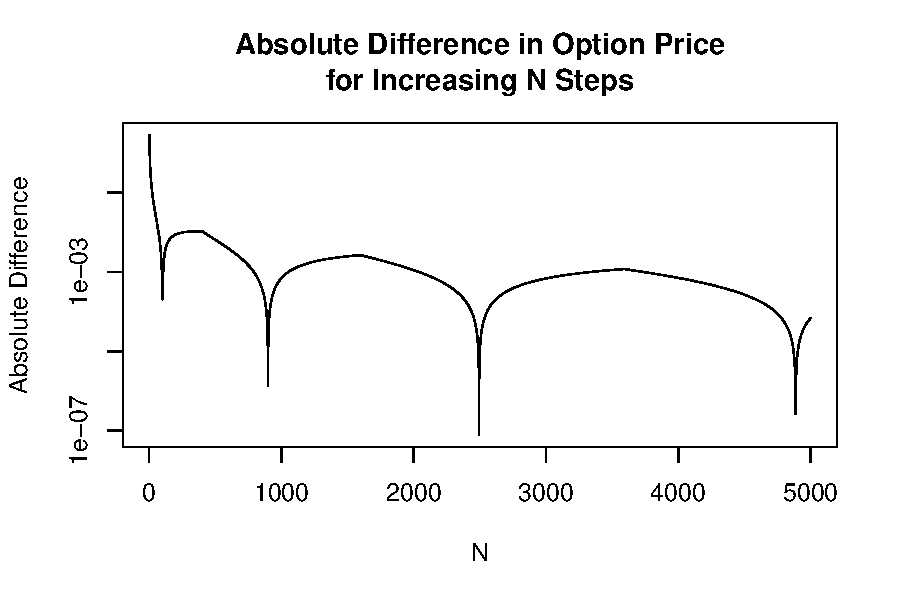
\includegraphics[scale=0.52]{../plots/price_conv_diff.pdf}
\caption{\footnotesize Increasing the value of $N$ leads to periodic behaviour in the additional precision for the prices given by the binomial model, with a decreasing trend.}
\end{figure}

\newpage
\appendix
\section{Code Output: Data Table}\label{sec:data}

{\small
\csvautolongtable{../macf_a4_final_code/implied_vols_googl_rounded.csv}
}
\newpage
\section{Code}\label{sec:code}
\subsection{main.cpp}
\lstinputlisting{../macf_a4_final_code/main.cpp}








\end{document}















